\section{Serge Haroche}

\begin{frame}[t]{Serge Haroche: In a Nutshell}
  \portraitpic{haroche.jpg}
  \vspace{3cm}
  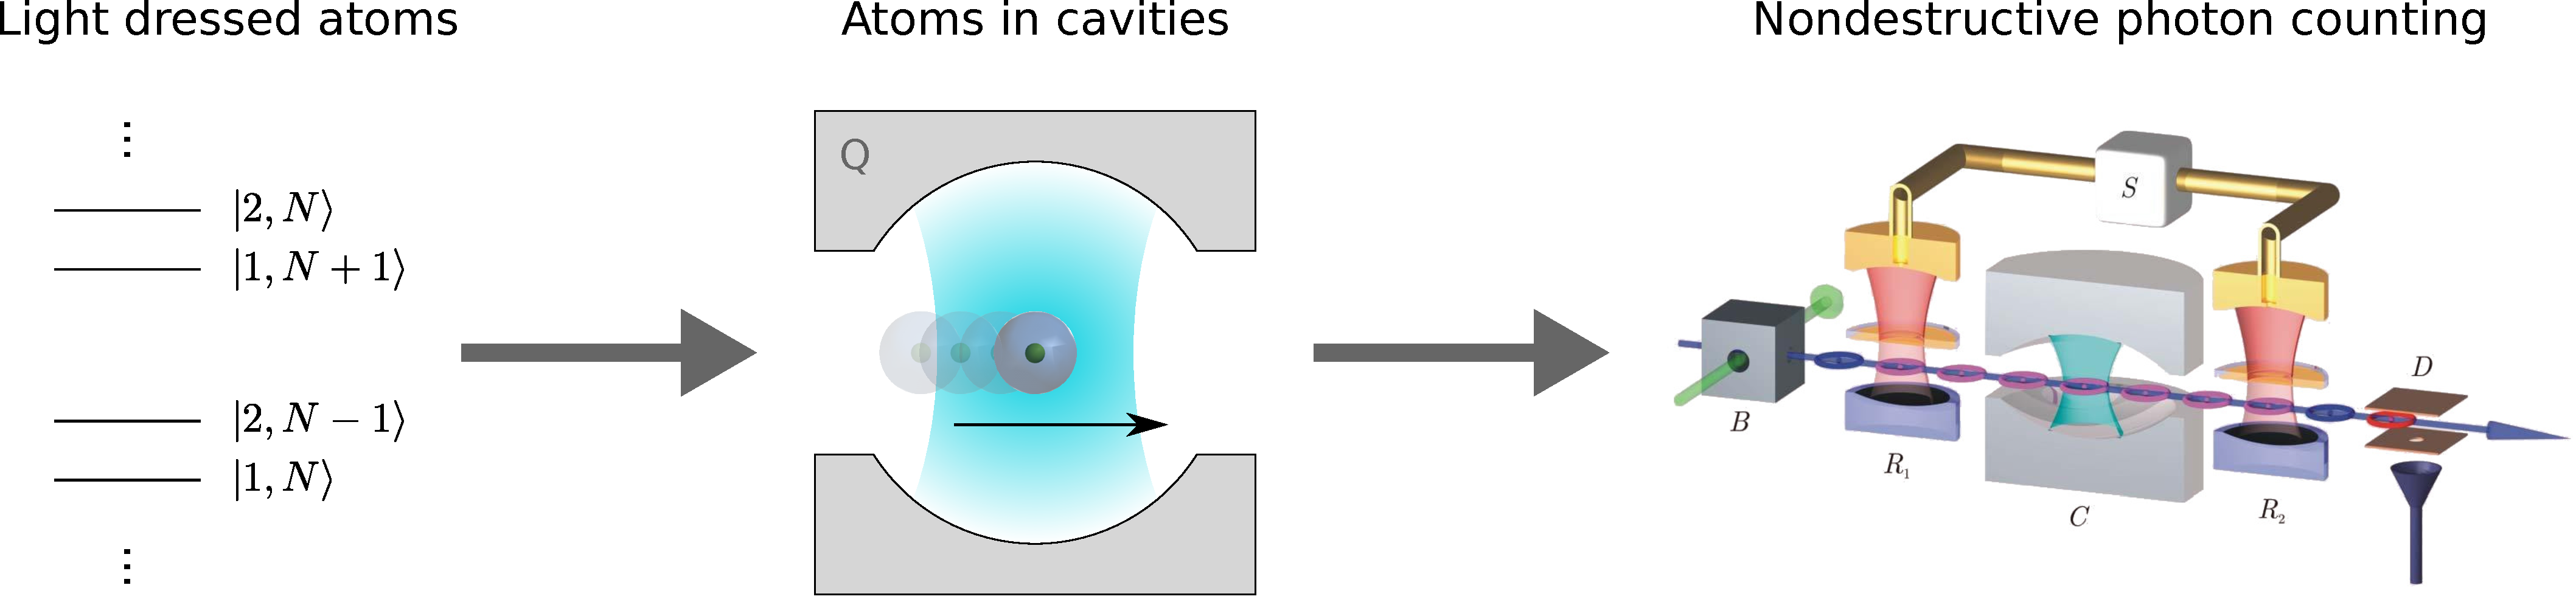
\includegraphics[width=\textwidth]{sh_nutshell.pdf}
\end{frame}

\begin{frame}[t]{Serge Haroche: Early life}
  \portraitpic{haroche.jpg}
  \visible<3>{
    \textpos{\linewidth}{0cm}{3cm}{\begin{quote}``I was a very good student,
    immediately at the head of my class in the Lycée Carnot''\end{quote}}
  }
  \visible<6>{\picpos{6cm}{1cm}{2.8cm}{lab_kastler_brossel.jpg}}
  \visible<7>{
    \textpos{\linewidth}{0cm}{3cm}{\begin{quote}``Enthralled by the mysterious beauty of the quantum
          world, it did not take me long to decide that I wanted to become a
        quantum physicist''\end{quote}}
  }

  \begin{minipage}[t][4cm][t]{\textwidth}
    \begin{itemize}
      \item<1-> Born in Casablanca, Morocco
      \item<2-> Parents move to Paris
      \item<4-> École préparatoires at Paris
      \item<5-> Accepted for École normale supérieure (ENS)
    \end{itemize}  
  \end{minipage}
  \begin{minipage}[t][0.2\textheight][t]{\textwidth}
    \begin{chronology}[10]{1940}{2016}{\textwidth}{5cm}
      \visible<1>{\event{1944}{24.02.1944}}
      \visible<2>{\event{1956}{'56}}                  
      \visible<4>{\event{1962}{'62}}                  
      \visible<5,7>{\event[1963]{1967}{'63 -- '67}}
      \visible<>{ \event[1967]{1972}{'67 -- '72}} 
      \visible<>{\event[1972]{1973}{'72 -- '73}}
      \visible<>{\event[1973]{1975}{'73 -- '75}}
      \visible<>{\event[1975]{1982}{'75 -- '82}}
      \visible<>{\event[1982]{2016}{'78-- now}}
    \end{chronology}
  \end{minipage}
\end{frame}

\begin{frame}[t]{Serge Haroche: Scientific Carreer}
  \portraitpic{haroche.jpg}
  \begin{minipage}[t][4.5cm][t]{\textwidth}
    \begin{itemize}
      \item PhD on light dressed atoms in optical pumping
      \item Supervisor: Claude Cohen-Tannoudji
      \picpos{2.5cm}{0.3cm}{1.5cm}{cohen-tannoudji.jpg}
      \picpos{7cm}{3cm}{1.2cm}{dressed_states.pdf}
    \end{itemize}  
  \end{minipage}
  \begin{minipage}[t][0.2\textheight][t]{\textwidth}
    \begin{chronology}[10]{1940}{2016}{\textwidth}{5cm}
      \event[1967]{1972}{'67 -- '72}
    \end{chronology}
  \end{minipage}
\end{frame}

\begin{frame}[t]{Serge Haroche: Scientific Carreer}
  \portraitpic{haroche.jpg}
  \visible<1>{
    \picpos{2.8cm}{1cm}{1.5cm}{arthur_schawlow_np.jpg}
    \picpos{2.8cm}{5cm}{1.5cm}{ted_haensch.jpg}
  }
  \visible<2>{\textpos{\linewidth}{0cm}{2.5cm}{\begin{quote}``After a few weeks in
  Stanford Art gave me a lab room and a pulsed dye laser and told me it was up
  to me to find something interesting to do with it.''\end{quote}}}
  \visible<3>{\picpos{9cm}{0.5cm}{1.9cm}{SH_quantum_beats_title.pdf}}
  %\visible<4>{\picpos{3.7cm}{0.5cm}{3cm}{v_type_quantum_beats.pdf}}
  %\visible<4>{\begin{textblock*}{3cm}(0.5cm,2.5cm)V-type\end{textblock*}}
  %\visible<4>{\picpos{4.8cm}{5.5cm}{3cm}{lambda_type_quantum_beats.pdf}}
  %\visible<4>{\begin{textblock*}{3cm}(5.5cm,2.5cm)$\Lambda$-type\end{textblock*}}
  %\visible<5->{\picpos{3.7cm}{0.5cm}{2cm}{SH_quantum_beats_plot.pdf}}
  %\visible<>{\picpos{5cm}{4.8cm}{2.5cm}{SH_quantum_beats_setup.pdf}}
  %\visible<5>{\picpos{5.5cm}{4.8cm}{2.8cm}{SH_quantum_beats_results.pdf}}
  \begin{minipage}[t][4.5cm][t]{\textwidth-1.9cm}
    \begin{itemize}
      \setlength\itemsep{0.9em}
      \item Postdoc at Arthur Schawlows Lab in Stanford
      \item<3-> Observation of quantum beats in Cs vapor
      \begin{quote}\end{quote}
    \end{itemize}  
  \end{minipage}
  \begin{minipage}[t][0.2\textheight][t]{\textwidth}
    \visible<1-3>{
    \begin{chronology}[10]{1940}{2016}{\textwidth}{5cm}
      \event[1972]{1973}{'72 -- '73}
    \end{chronology}
  }
  \end{minipage}
\end{frame}

\begin{frame}[t]{Serge Haroche: Scientific Carreer}
  \portraitpic{haroche}
  \begin{minipage}[t][4.5cm][t]{\textwidth-1.9cm}
    \begin{itemize}
      \setlength\itemsep{0.9em}
      \item Budget and laboratory at ENS: Beginning of experimental studies of Rydberg atoms 
      \item<2-> Full professor at Université Paris VI
      \item<3-> Professorship and research at Yale {\em and} ENS
      \item<4-> Professor at Collège de France
      \item<5-> Gold medal of the Centre national de la récherche scientifique
        (CNRS)
    \end{itemize}  
  \end{minipage}
  \begin{minipage}[t][0.2\textheight][t]{\textwidth}
    \begin{chronology}[10]{1940}{2016}{\textwidth}{5cm}
      \visible<1>{\event{1973}{'73}}
      \visible<2>{\event{1975}{'75}}
      \visible<3>{\event[1984]{1993}{'84 -- '93}}
      \visible<4>{\event{1999}{'99}}
      \visible<5>{\event{2009}{'09}}
    \end{chronology}
  \end{minipage}
\end{frame}


\begin{frame}[t]{Serge Haroche: CQED}
  \portraitpic{haroche}
  \visible<4,6>{\source{{PhysRevLett, inkscape}}}
  \visible<1>{\picpos{4cm}{.5cm}{1.5cm}{atom_in_cavity.pdf}}
  \visible<2>{\picpos{4cm}{.5cm}{1.5cm}{atom_in_cavity_res.pdf}}
  \visible<2>{\begin{textblock*}{5.5cm}(5cm,2.5cm)Resonant case $$\Gamma_{res} =
    \Gamma_0 \, \frac{3Q\lambda^3}{4\pi^2V}$$ $\rightarrow$ enhanced spontaneous
    emission\end{textblock*}}
  \visible<3>{\picpos{9cm}{0.5cm}{2.5cm}{SH_cavity_enhanced_em_title.pdf}}
  \visible<4->{
    \picpos{5cm}{0.5cm}{1.5cm}{SH_cavity_enhanced_em_setup.pdf}
    \textpos{3cm}{0.3cm}{3.6cm}{\small 23S}
  }
  \visible<4>{\textpos{3cm}{5.55cm}{4.7cm}{\small 23S or 22P?}}
  \visible<5>{\picpos{4.5cm}{5.55cm}{2.8cm}{SH_ionization_detection.pdf}}
  \visible<6>{\picpos{5.5cm}{5.55cm}{3.5cm}{SH_cavity_enhanced_em_results.pdf}}
    
  \begin{minipage}[t][4.5cm][t]{\textwidth-1.5cm}
    \begin{itemize}
      \item Cavity QED (CQED): what happens to atoms in cavities?
    \end{itemize}  
  \end{minipage}
  \begin{minipage}[t][0.2\textheight][t]{\textwidth}
    \visible<3>{
    \begin{chronology}[10]{1940}{2016}{\textwidth}{2cm}
      \visible<3>{\event{1983}{'83}}
      \visible<>{\event{1999}{'99 -- '99}} %this will never be visible, just
        % takes care of spacing
    \end{chronology}
  }
  \end{minipage}
\end{frame}

\begin{frame}[t]{Serge Haroche: CQED}
  \portraitpic{haroche}
  \visible<1>{\picpos{4cm}{.5cm}{1.5cm}{atom_in_cavity.pdf}}
  \visible<2>{\picpos{4cm}{.5cm}{1.5cm}{atom_in_cavity_cut.pdf}}
  \visible<2>{
    \begin{textblock*}{5.5cm}(5cm,2.8cm) Polarization dependend ``cut-off'' of
      vacuum modes \end{textblock*}
    \textpos{5.5cm}{5.3cm}{3.9cm}{$\rightarrow$}
    \textpos{5.5cm}{5.75cm}{3.75cm}{supression of spontaneous
    emission}
    }
  \visible<3>{\picpos{9cm}{0.5cm}{1.5cm}{SH_supression_spont_em_title.pdf}}
  %\visible<4->{
  %  \picpos{5.5cm}{0.5cm}{2cm}{SH_supressed_spont_em_setup.jpg}
  %}
  %\visible<4-5,7-8>{\picpos{4cm}{6.3cm}{3cm}{SH_supression_spont_em_scheme.pdf}}
  %\visible<6>{\picpos{6cm}{6.3cm}{3cm}{SH_supression_spont_em_scheme2.pdf}}
  %\visible<5>{
  %  \picpos{5.5cm}{0.5cm}{2cm}{SH_supressed_spont_em_setup_1.pdf}
  %  \textpos{2.5cm}{-0.4cm}{4.1cm}{\scriptsize Excitation to 7P$_{3/2}$ and decay
  %    to 5D$_{3/2}$}
  %  }
  %\visible<6>{
  %  \picpos{5.5cm}{0.5cm}{2cm}{SH_supressed_spont_em_setup_2.pdf}
  %  \textpos{3.6cm}{2.5cm}{6cm}{\scriptsize Flight through cavity\\ $\approx
  %13$ natural lifetimes}
  %  }
  %\visible<7>{
  %  \picpos{5.5cm}{0.5cm}{2cm}{SH_supressed_spont_em_setup_3.pdf}
  %  \textpos{3cm}{3.8cm}{5.65cm}{\scriptsize Excitation to 26F}
  %  }
  %\visible<8>{
  %  \picpos{5.5cm}{0.5cm}{2cm}{SH_supressed_spont_em_setup_4.pdf}
  %  \textpos{3cm}{4.1cm}{5.65cm}{\scriptsize Ionization detection\\ of 26F}
  %  }
  %\visible<9>{\picpos{4cm}{6cm}{2.5cm}{SH_supression_spont_em_results.pdf}}
    
  \begin{minipage}[t][4.5cm][t]{\textwidth-1.5cm}
    \begin{itemize}
      \item Cavity QED (CQED): what happens to atoms in cavities?
    \end{itemize}  
  \end{minipage}
  \begin{minipage}[t][0.2\textheight][t]{\textwidth}
    \visible<3>{
    \begin{chronology}[10]{1940}{2016}{\textwidth}{2cm}
      \visible<3>{\event{1987}{'87}}
      \visible<>{\event{1999}{'99 -- '99}} %this will never be visible, just
        % takes care of spacing
    \end{chronology}
  }
  \end{minipage}
\end{frame}

\begin{frame}[t]{Serge Haroche: QND Measurement}
  \portraitpic{haroche}
  \visible<2>{\source{Nature99}}
  \visible<3>{\source{arXiv}}
  \visible<2>{\picpos{6cm}{2cm}{2.9cm}{SH_single_photon_detection_title.pdf}}
  \visible<3>{\picpos{8cm}{1cm}{3.9cm}{sh_super_high_q_title.pdf}}
  \begin{minipage}[t][4.5cm][t]{\textwidth-1.5cm}
    \begin{itemize}
      \item Quantum non-demolition (QND) measurement: can we observe photons
        without destroying them?
      \item<2-> Probe photon field with  slightly off-resonant Rydberg atom
      \item<3-> Breakthrough: super-high-Q cavity to store photons for
        $\approx\,$0.1\,s $\equalhat$ 30000\,km
    \end{itemize}  
  \end{minipage}
  \begin{minipage}[t][0.2\textheight][t]{\textwidth}
    \visible<2-3>{
    \begin{chronology}[10]{1940}{2016}{\textwidth}{2cm}
      \visible<2>{\event{1999}{'99}}
      \visible<3>{\event{2006}{'06}}
      \visible<>{\event{1999}{'99 -- '99}} %this will never be visible, just
        % takes care of spacing
    \end{chronology}
  }
  \end{minipage}
\end{frame}

\begin{frame}[t]{Serge Haroche: QND Measurement}
  \portraitpic{haroche}
  \source{{Nobel Lecture S. Haroche, inkscape}}
  \visible<1->{\picpos{7cm}{0cm}{1cm}{sh_photon_detection_background.pdf}}
  \visible<1->{\picpos{5cm}{7cm}{3cm}{rabi_cycle.pdf}}
  
  \visible<2>{\picpos{7cm}{0cm}{1cm}{sh_photon_detection_1.pdf}}
  \visible<2>{\picpos{5cm}{7cm}{3cm}{rabi_cycle_1.pdf}}
  \visible<2>{\textpos{4cm}{0.6cm}{4.8cm}{\small creation of Rydberg state
  $\ket{e}=\ket{51}$}} 

  \visible<3>{\picpos{7cm}{0cm}{1cm}{sh_photon_detection_2.pdf}}
  \visible<3>{\picpos{5cm}{7cm}{3cm}{rabi_cycle_2.pdf}}
  \visible<3>{\textpos{4cm}{1.2cm}{4.8cm}{\small $\pi /2$-pulse}} 
  
  \visible<4>{\picpos{7cm}{0cm}{1cm}{sh_photon_detection_3.pdf}}
  \visible<4>{\textpos{6cm}{1.2cm}{4.8cm}{\small Rabi induced phase shift $ \Phi=
\begin{cases} 0 & \text{if no photon}\\ \pi  & \text{if one photon} \end{cases}$ }} 
  
  \visible<5>{\picpos{7cm}{0cm}{1cm}{sh_photon_detection_4.pdf}}
  \visible<5>{\textpos{4cm}{1.2cm}{4.8cm}{\small $\pi /2$-pulse $\ket{\psi} =
\begin{cases} \ket{g} & \text{if no photon}\\ \ket{e}  & \text{if one photon} \end{cases}$}} 
  
  \visible<6>{\picpos{7cm}{0cm}{1cm}{sh_photon_detection_5.pdf}}
  \visible<6>{\textpos{4cm}{1.7cm}{4.8cm}{\small ionization detection\\ $\ket{g}$
  or $\ket{e}$}} 

  \begin{minipage}[t][4.5cm][t]{\textwidth-1.5cm}
    \begin{itemize}
      \item Quantum non-demolition measurement scheme
    \end{itemize}  
  \end{minipage}
  \begin{minipage}[t][0.2\textheight][t]{\textwidth}
    \visible<>{
    \begin{chronology}[10]{1940}{2016}{\textwidth}{2cm}
      \visible<2>{\event{1999}{'99}}
      \visible<3>{\event{2006}{'06}}
      \visible<>{\event{1999}{'99 -- '99}} %this will never be visible, just
        % takes care of spacing
    \end{chronology}
  }
  \end{minipage}
\end{frame}

\begin{frame}[t]{Serge Haroche: QND Photon counting}
  \portraitpic{haroche}
  \visible<2>{\source{Nature07}}
  \visible<1>{\picpos{8cm}{0.5cm}{1.5cm}{SH_photon_quantum_jumps_title.pdf}}
  \visible<2>{\picpos{6cm}{0.5cm}{1.5cm}{SH_photon_quantum_jumps_results.pdf}}
  \visible<2>{\textpos{\textwidth}{0.5cm}{5.5cm}{$\rightarrow$ photon ``born'' in
  vacuum survives in cavity for 0.5\,s, measured by several hundreds of atoms}}

  \begin{minipage}[t][4.5cm][t]{\textwidth-1.5cm}
    \begin{itemize}
      \item Black body photon quantum jumps
    \end{itemize}  
  \end{minipage}
  \begin{minipage}[t][0.2\textheight][t]{\textwidth}
    \visible<1>{
    \begin{chronology}[10]{1940}{2016}{\textwidth}{2cm}
      \visible<1>{\event{2007}{'07}}
      \visible<>{\event{1999}{'99 -- '99}} %this will never be visible, just
        % takes care of spacing
    \end{chronology}
  }
  \end{minipage}
\end{frame}

%\begin{frame}[t]{Serge Haroche: QND Photon counting}
%  \portraitpic{haroche}
%  \visible<1>{\picpos{8cm}{0.5cm}{1.5cm}{SH_field_state_collapse_title.pdf}}
%  \visible<2>{\picpos{9cm}{0.5cm}{1.5cm}{SH_field_state_collapse_results.pdf}}
%  \visible<2>{\textpos{\textwidth}{0.5cm}{5.5cm}{$\rightarrow$ wavefunction collapse from
%  quantum fluctuation to ``classical'' single mode occupation}}
%
%  \begin{minipage}[t][4.5cm][t]{\textwidth-1.5cm}
%    \begin{itemize}
%      \item Photon number wavefunction in cavity
%    \end{itemize}  
%  \end{minipage}
%  \begin{minipage}[t][0.2\textheight][t]{\textwidth}
%    \visible<1>{
%    \begin{chronology}[10]{1940}{2016}{\textwidth}{2cm}
%      \visible<1>{\event{2007}{'07}}
%      \visible<>{\event{1999}{'99 -- '99}} %this will never be visible, just
        % takes care of spacing
%    \end{chronology}
 % }
%  \end{minipage}
%\end{frame}
